%!TEX root = ../A_Novel_Filtering_Approach_for_Robust_and_Fast_Keypoint_Matching_in_Mobile_Environment.tex


\section{Proposed Method}

%In this paper, we proposed a keypoint filtering method by means of evaluation of detected keypoint with regard to the matching quality. 

% In this paper, we propose a keypoint filtering method to store better keypoints while online matching stage. To determine which keypoint is better, we propose a score function to evaluate 

% 본 논문에서는 online matching 단계에서의 매칭 품질을 향상시키기 위해서 매칭에 좋은 특징점들만을 저장하는 keypoint filtering 알고리즘을 제안한다. 이를 위하여 online 학습 단계에서 추출된 특징점들의 

% a detected keypoint is good to store or not. 
% 본 논문에서는 matching quality 를 기준으로 detected keypoint 를 evaluate하여 filtering하는 방법을 제안한다. 이를 통하여 matching quality가 높은 점들만을 학습함으로써 online matching 과정에서 높은 matching preciseness와 빠른 속도를 얻을 수 있다. 본 장에서는 matching quality 에 따라서 keypoint를 evaluation 하기 위한 criteria 를 정의하고, ground truth data 를 기준으로 이러한 criteria 가 동작됨을 증명한다. 또한, 이러한 기준에 의하여 분류된 keypoint 들의 image patch 를 비교하여 matching에 좋은 특징점과 그렇지 않은 특징점의 xxx 측면에서의 차이점을 비교하였다.

본 논문에서는 특징점 매칭


asdfasdf  

%!TEX root = ../A_Novel_Filtering_Approach_for_Robust_and_Fast_Keypoint_Matching_in_Mobile_Environment.tex

\subsection{Problem}
In general, keypoint matching methods 
일반적으로 키포인트 기반의 매칭 방법은 미리 학습된 키포인트 데이터베이스 $K^R$와 입력된 영상을 분석하여 생성된 키포인트 집합 $K^I$를 비교하여, 가장 유사한 키포인트 pair 집합 $C = \{(k_i^R, k_j^I) | \argmin\limits_{k_i\in K^R}  \argmin\limits_{k_j\in K^I} | k_i^R - k_j^I | \}$ 을 계산하는 과정이다. 기존의 키포인트 매칭 방법은 검출된 키포인트 집합 $K^R$을 그대로 사용하였으나, 본 논문에서는 키포인트 평가 함수($s(k)$)를 제안하여 이러한 평가 함수에 의하여 필터링된 집합 $K' = \{ k | s(k) is\;\; high \} \in K^R$ 을 계산하고, 이러한 필터링 된 부분집합 $K'$는 필터링 되지 않은 $K^R$에 비하여 더 높은 인식성능을 보여줌을 증명하고자 한다. \texttt{조금만 더 늘여쓰자}

%!TEX root = ../A_Novel_Filtering_Approach_for_Robust_and_Fast_Keypoint_Matching_in_Mobile_Environment.tex

\subsection{Keypoint Score Function}
%feature matching 기반의 증강현실 시스템에서는 online process 이전에 reference images들을 오프라인으로 학습(train)하여 비교 대상인 feature database 를 생성하게 된다. 특히 앞의 matching data structure 연구에서 보듯이 온라인 인식의 성능을 높이기 위하여 오프라인 처리에서 다양한 연산을 적용하여 매칭 구조체를 구성함으로써 온라인 인식의 속도나 인식율을 높이기 위한 방법도 제안되고 있다. 
%이러한 기존의 특징점 매칭 방법들은 Feature Detection 알고리즘에서 검출한 특징점을 단순히 모두 학습에 사용하였다. 하지만, 특징점 검출 알고리즘은 Description 알고리즘과 독립적으로 수행되기 때문에 검출(Detect)된 특징점들에 대한 Descriptor가 매칭 성능을 보장할 수 없다는 문제가 있다. 

General keypoint matching generates the feature database, the subjects of comparison, by way of the offline training of the reference images before online matching procedure. \texttt{In particular, as shown in the foregoing study of matching data structure, a method that composes a matching structure by applying a various computations to offline process to increase the online recognition speed and recognition rate is proposed.} Such established kaypoints matching methods used simply all of the keypoints detected in feature detection module for training. However, since the feature detection algorithm is performed independently from the description algorithm, the descriptor is not able to ensue the matching performance for the detected features. \texttt{이유를 들라}

%따라서 본 논문에서는 오프라인 학습 과정에서 학습 대상 특징점을 평가하고, 이를 통하여 실시간 인식에 강인한 성능을 제공하는 특징점만을 선정하였다. 이러한 특징점들만을 데이터베이스에 저장함으로써 인식 품질을 유지하면서도 인식 속도를 향상시킬 수 있는 방법을 제안한다.

Thus, in this paper, the keypoints of the subjects of training in the offline training process were assessed \texttt{and only the keypoints providing rigid real-time recognition performance were selected.} Accordingly, both recognition rate and speed can be enhanced by only saving discriminant (good) features in the database based on proposed method.


\subsubsection{Definition of Good Keypoints}

%제안하는 방법은 detect된 특징점을 분석하여 인식에 좋은 정도를 측정함으로써 좋은 특징점만을 filtering 한다. 이를 위하여 좋은 특징점을 정의하였다.

The proposed filtering method selects only good keypoints by analyzing the characteristics of detected keypoints and measuring the degree of effectiveness for image matching. 

There are several factors which good keypoints should follows:

%첫 번째 인식에 좋은 특징점의 조건은 대상 영상이 다양하게 변화되는 환경에서도 안정적으로 특징점으로 검출되어야 한다는 점이다. 실제 온라인 매칭 과정에서 입력되는 카메라 영상에는 인식하고자 하는 대상 영상이 회전이나 크기, perspective, 노이즈, 조명 등의 다양한 형태의 변환이 적용되어 있다. 인식에 좋은 특징점은 이러한 변환된 영상에서도 안정적으로 특징점이 검출이 됨으로써 Descriptor를 생성할 수 있도록 하는 점이어야 한다.
\textit{Repeatability}: Good keypoints need to be stably detected even in various environment. In actual matching environments, a wide range of transformed image degradation may occurred, such as the rotation, size, noise and lighting of the targeted images. The good keypoints have to be stably extracted against those transformation.

%이러한 안정적 특징점 검출은 Repeatability Score로 측정이 가능하다. Repeatability는 아래 그림과 같이 전체 변환된 영상의 개수 대비 변환된 영상에서 키포인트가 변환되어 존재하는 경우의 비율로 계산된다.
The detection of stable keypoints can be measured by \textit{Repeatability} condition. \textit{Repeatability} is calculated by the ratio between the \texttt{total number of synthesized images and the number of cases where the transformed keypoints are existent in the synthesized images. }


\begin{equation}
p_{rep}(p_i) = \frac{n_i^{overlap}}{N}
\end{equation}

% 여기에서 $n_i^{overlap}$는 변환된 영상($T_t(I)$)의 키포인트 집합($K_t'$)에 키포인트($p_i$)가 변환된 점이 존재($T(p_i)\in K_t'$)하는 횟수로 계산되며, $N$은 총 변환된 영상의 개수로 모든 키포인트가 동일한 값을 가지게 된다.

\noindent
where $p_{rep}(p_i)$ represents repeatability score of given point $p_i$, $n_i^{overlap}$ is calculated by the frequency of the existence of transformed keypoint($p_i$) in the set of keypoints($T(p_i)\in K_t'$) of synthesized images $T_t(I)$; $N$ is the total number of synthesized images ; and all keypoints have single value. 

%두 번째 인식에 좋은 특징점 집합의 조건은 해당 키포인트가 변화된 영상에서 만들어진 descriptor와의 매치가 실패가 적어야 한다(Similarity)는 점이다.
%이는 해당 특징점의 Sensitivity(True Positive Rate)와 연관이 있다. Reference 영상의 어떤 특징점($p_i$)에 대하여 학습 과정에서 다양하게 변환된 영상($T_t(I)$)에서의 모든 키포인트 집합($K_t'$)의 Descriptor 사이의 매칭을 계산하여 해당 특징점에 대한 Genuine 분포와 Impostor 분포를 계산할 수 있다. 이 때, 해당 키포인트가 변화된 영상에서의 Descriptor와의 매치가 실패가 적기 위해서는, Genuine 분포가 매치 임계 거리(Match Distance Threshold)에서부터 충분히 떨어져 작은 값을 가져야 한다. 이를 위하여 Genuine 분포의 평균을 이용하여 이를 측정하였다. 식 \ref{eq:similarity}에서 보는 것과 같이, Genuine 분포가 작을 수록 좋은 특징점이기 때문에 genuine 분포의 평균을 normalize 하여 1에서 뺌으로써 평가 함수를 계산하였다.

\textit{Similarity}: Good keypoints need to be well-matched with identical keypoints even though targeted images change in various ways. With regard to a certain keypoint($p_i$) of reference images, genuine distribution' and imposter distribution' for the corresponding keypoint can be measured by calculating the matching between the descriptors of all the sets of keypoints($p_i$) in images($T_t(I)$) transformed in various ways  during the training process. At this time, to reduce the failure in matching the corresponding keypoints and the descriptors in the transformed images, the genuine distribution needs to have small value, being far enough away from match distance threshold. To this effect, it was measured using the mean of genuine distribution. As shown in Equation \eqref{eq:similarity}, the keypoints with the decreasing the genuine distribution are better, so the evaluation function was calculated by normalizing the mean of the genuine distribution and subtracting its value from 1.  

\begin{equation} \label{eq:similarity}
p_{sim}(p_i) = 1 - \frac{\mu_{gen,i} - \min_i \mu_{gen,i}}{\max_i \mu_{gen, i} - \min_i \mu_{gen,i}}
\end{equation}	
where $p_{sim}(p_i)$ represents similarity score of given point $p_i$, $\mu_{gen, i}$ represents mean of genuine distribution of give point $p_i$. 

%세 번째 조건은 학습된 특징점이 자신과 다른 특징점과는 매치가 이루어지지 않아야 한다(Separability)는 점이다. 이는 각 특징점의 Impostor 분포와 관련이 있다. 다양하게 변화된 영상에서 추출된 특징점 중 자기 자신이 변환된 특징점이 아닌 다른 특징점들과의 매칭 분포를 Impostor 분포라 한다. 어떤 특징점이 자신 이외의 다른 키포인트와 낮은 매칭 성공률을 보여주기 위해서는 Genuine 분포와 Impostor 분포가 잘 구분이 되어야 한다.
%이를 위하여 본 논문에서는 Fisher's Discriminant Ratio\cite{fisher_use_1936}를 이용하였다. 이는 1-dimensional, two class problem에서 sample의 평균과 분산에 의하여 두 클래스 사이의 거리를 측정하는 방식이다. 두 번째 Similarity 조건에 의하여 Genuine 분포가 충분히 작음이 보장이 되었기 때문에 Impostor의 분포가 Genuine 분포에 비하여 충분히 떨어져 있다면 Impostor 분포에 존재하는 특징점들과는 매치가 이루어지지 않음이 보장된다. separability 값 역시 수식 \ref{eq:norm_separability}과 같이 normalize 과정이 필요하다.

\textit{Separability}: The trained keypoints and other keypoints shall not be matched, which is associated with the imposter distribution of each keypoint. Of the keypoints extracted from the images converted in various images, the distribution of the matching with other keypoints rather than the converted keypoints themselves are referred to as imposter distribution. Thus for a specific keypoint to show the low success rate of matching with other keypoints rather than themselves, in is necessary that the genuine distribution and imposter distribution are well classified. To this effect, in this paper, \textit{Fisher's Discriminant Ratio\cite{fisher_use_1936}} was used. It measures the distance between two classes by the mean and distribution of sample in 1-dimensional, two class problems. Since the second Similarity condition ensures the genuine distribution is small enough, the nonexistence of the matching with the keypoints in the imposter distribution is ensured if the importer distribution is far enough away compared with the genuine distribution. Separability value also requires the normalization process as shown in equation \eqref{eq:norm_separability}.  


\begin{equation}
FDR(p_i) = \frac{(\mu_{gen,i} - \mu_{imp, i})^2}{\sigma_{gen, i}^2 + \sigma_{imp, i}^2}
\end{equation}
\begin{equation}\label{eq:norm_separability}
p_{sep}(p_i) = \frac{FDR(p_i) - \min_i {FDR(p_i)}}{\max_{i} {s_i}}
\end{equation}	
where $p_{sep}(p_i)$ represents similarity score of given point $p_i$, $\mu_{gen, i}, \mu_{imp, i}$ represent mean of genuine and impostor distribution of give point $p_i$, respectively. $\sigma_{gen,i}, \sigma_{imp, i}$ represent standard deviation of genuine and impostor distribution, respectively.


%이렇게 계산된 세가지 criteria를 이용하여 각 특징점의 score function을 정의할 수 있다. 세 조건은 종속이므로 식 \ref{eq:score_function}와 같이 정의된다.

The score functions of each keypoint can be defined using 3 criteria calculated as above. The 3 conditions are dependent, so can be defined as shown in Equation \eqref{eq:score_function}. 

\begin{equation}\label{eq:score_function}
gf(p_i) = p_{rep}(p_i)p_{sim}(p_i)p_{sep}(p_i)
\end{equation} 



% \subsubsection{}
%%%%% 시간이 되면 실험 부분을 추가하자 %%%%%


%!TEX root = ../A_Novel_Filtering_Approach_for_Robust_and_Fast_Keypoint_Matching_in_Mobile_Environment.tex

\subsection{Proof of Criteria}
\subsubsection{Validation Design}
% 제안하는 keypoint evaluation criteria 를 검증하기 위하여, 우리는 각 keypoint 들의 correct matching count 를 기준으로 제안된 criteria의 연관성을 측정하였다. 먼저, 우리는 robust image matching 환경을 고려하여, 다양한 변환을 적용한 dataset을 생성하였다. 그리고 이러한 dataset을 기반으로, 각 keypoint 별로 correct matching count 를 측정하여 matching quality 에 대한 ground truth data를 계산하였다.
To validate the proposed keypoint evaluation criteria, we examined a relationship between criteria and correct matching count of each keypoints. At first, to provide robust image matching, we synthesized image dataset by various image transformation. Then, based on this dataset, we counted correct matching count for each keypoint, and this correct matching count is a basis of matching quality. 이러한 correct matching count가 높은 특징점은 fixed image dataset 에서 더 높은 matching quality를 보여준다고 볼 수 있기 때문에 본 논문에서 제안하는 Matching에 더 적합한 keypoint로 볼 수 있다. 반대로 correct matching count가 낮은 특징점은 특징점이 반복적으로 검출되지 않거나, 모호성이 높아 inter-keypoint miss-match가 많이 발생하는 특징점으로 matching에 적합하지 못한 keypoint로 볼 수 있다. 따라서, 이러한 correct match count 와 제안하는 keypoint evaluation score function (see, Eq. \ref{eq:score_function}) 간의 상관관계를 관찰함으로써 제안하는 score function 의 적절성을 검증할 수 있다.

% Genuine / Impostor 분포에 관한 얘기

\subsubsection{Dataset}
검증에 사용된 이미지는 서울 관광 가이드북\cite{_seoul_2014}의 \textit{Seoul Tour Map} 16장을 사용하였다. 우리는 이러한 이미지를 대상으로 rotate($0.5-2.0$-folds, at the interval of 0.1-fold), scaling($0\degree-360\degree$, at the interval of $10$ intervals), and blurring (Gaussian blur, $r \in \left \{ 0, 3, 5, 7 \right \}$ pixels) 의 transform을 적용하여 총 36,864 장의 dataset을 생성하였다. 이 중 랜덤으로 training Set 16,114 장, Test set 16,142 장을 선택하여 실험을 진행하였다. 

\subsubsection{Images Patches}
그림 \ref{fig:image_patches}와 같이, correct matching count 를 기준으로 상위 10개의 keypoint 와 하위 10개의 keypoint 들의 특징을 비교하였다. 상위 10개에 대한 패치는 비교적 단순한 사각형 형태에서 많이 검출되었다. Genuine과 Impostor Histogram의 값을 정규화하여 표현된 Normal Distribution의 분포를 보면 Genuine과 Impostor 분포가 확연하게 구분되는 것을 확인할 수 있다. 반면, 하위 10개에 대한 패치는 글자 또는 단순한 패턴이 반복되는 형태에서 많이 검출되었다. Genuine과 Impostor Histogram의 값을 정규화하여 표현된 Normal Distribution의 분포를 보면 Genuine과 Impostor 분포가 많은 부분 겹쳐있어 구분이 어려운 것을 확인할 수 있다. 
인식에 좋은 특징점은 큰 숫자 패치와 같이 단순한 색상으로 패턴이 큰 숫자 표지와 같은 특징점이 인식에 좋은 성능을 보여주었으며, 반대로 작은 설명 글씨와 같은 특징점들은 인식 성능이 좋지 못하였으며, 이러한 점들을 제거하고 학습을 수행하는 것이 좋다.


\begin{figure}[htb!]
  \centering     %%% not \center
    \subfloat[the best 100-images]{\label{fig:patches_good}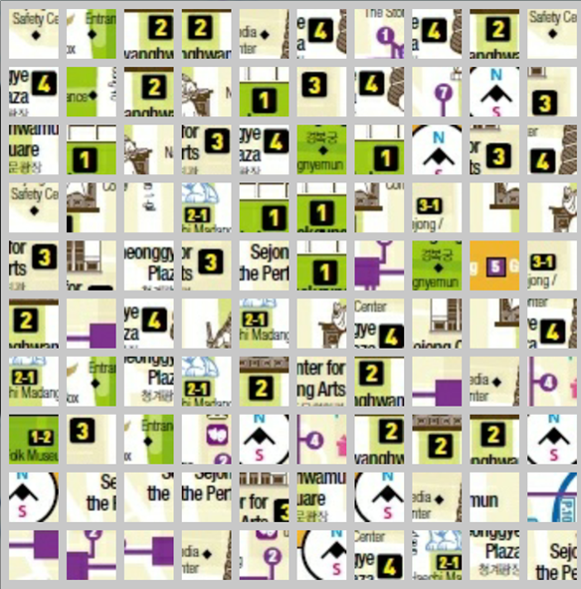
\includegraphics[width=0.45\textwidth]{3_proposed/patch_good}}
    % 
\\
    \subfloat[the worst 100-images]{\label{fig:patches_bad}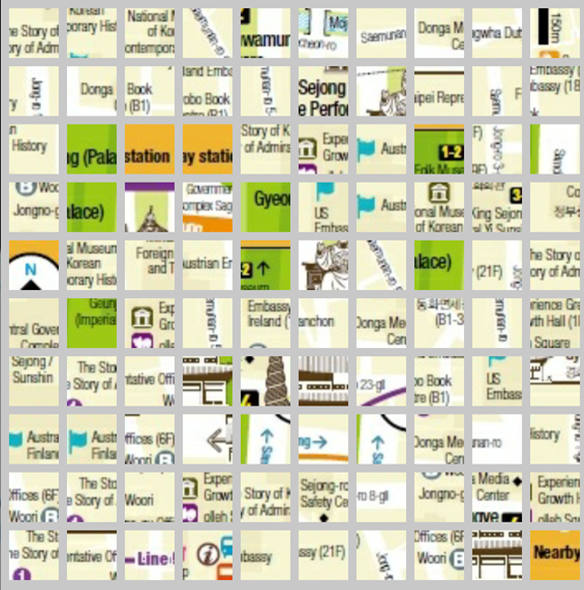
\includegraphics[width=0.45\textwidth]{3_proposed/patch_bad}}
  \caption{The Best/Worst 100-Images with Regard to Correct Matching Count}
    \label{fig:image_patches}
\end{figure}


